\chapter{Application to cloud microphysics}

\section{Mathematics Model and numerical implementation}
Similar to most previous DNS, our new DNS is based on the incompressible
Boussinesq fluid system \cite{And04}. Briefly, the temperature $T$ and vapor
mixing ratio $q_v$ are described by the following equations (\cite{Kumar11}):

\begin{equation}
\partial_{t}T+(\mathbf{u}\cdot\nabla)T=\frac{L_{h}}{c_{p}}C_{d}+\mu_{T}\nabla^{2}T\label{eq:Temp}
\end{equation}

\begin{equation}
\partial_{t}q_{v}+(\mathbf{u}\cdot\nabla)q_{v}=-C_{d}+\mu_{v}\nabla^{2}q_{v}\label{eq:Vapor}
\end{equation}

where $L_{h}$ is the latent heat of water vapor condensation,
$c_{p}$ is the specific heat at constant pressure, $\mu_{T}=\mu_{v}$ are
the molecular diffusivity for temperature and water vapor, respectively
and assumes to be equal. The condensation rate $C_{d}$ denotes the rate of exchange between liquid and vapor, and is described by:

\begin{subequations}

\begin{equation}
C_{d}(\mathbf{X},t)=\frac{d(m_{l}(\mathbf{X},t))}{m_{a}dt}=\frac{4\pi\rho_{l}K}{\rho_{0}a^{3}}\Sigma_{i=1}^{n}S(\mathbf{X}_{i},t)R_{i}(t)\label{eq:CondRate}
\end{equation}


where $K$ is a function of temperature and pressure given by:

\begin{equation}
K=1/[(\frac{L_{h}}{R_{v}T}-1)\frac{L_{h}\rho_{l}}{C_{T}T}+\frac{\rho_{l}R_{v}T}{De_{s}(T)}]\label{eq:CondCoeff}
\end{equation}


where $R_{v}$ is the individual gas constant, 
$C_{T}$ is the coefficient of thermal conductivity, $e_{s}(T)$ is
the saturation vapor pressure. The supersaturation $S(X,t)$ is calculated
directly from the water vapor mixing ratio and temperature from the following
equation

\begin{equation}
S(\mathbf{X},t)=\frac{q_{v}(\mathbf{X},t)}{q_{v,s}(\mathbf{X},t)}-1\label{eq:Supersat}
\end{equation}

\end{subequations}

where $q_{v,s}$ is the corresponding saturated water vapor mixing ratio. The droplets
will grow or shrink depending on the sign of supersaturation $S$.

The liquid water mixing ratio is given by
\begin{equation}
q_{c}(\mathbf{X},t)=\frac{4\pi\rho_{l}}{3\rho_{0}a^{3}}\sum_{i=1}^{n}R_{i}^{3}(t)\label{eq:cloud_water}
\end{equation}


where $a$ is the size of a grid cell, $n$ is the number of droplets
in the grid cell; $\rho_{l}$ and $\rho_{0}$ are the densities of water
and air. $R_{i}(t)$ is the radius of the $i$-th droplet.

The dynamical field is given by
\begin{subequations}

\begin{equation}
\partial_{t}\mathbf{u}+(\mathbf{u}\cdot\nabla)\mathbf{u}=-\frac{1}{\rho_{0}}\nabla p+\nu\nabla^2 \mathbf{u}+\mathbf{f}_b + \mathbf{f}_e\label{eq:NS1}
\end{equation}


\begin{equation}
\nabla\cdot \mathbf{u}=0\label{eq:NS2}
\end{equation}

\end{subequations}

where $\nu$ is the kinetic viscosity, $\rho_{0}$ is the density of
dry air, $\mathbf{u}$ is the velocity field, $p$ is the pressure field. Here $\mathbf{f}_b$ is the force immitating the buoyancy effects and $\mathbf{f}_e$ is the external low-wavenumber forcing:
\begin{equation}
\mathbf{f}_b= 
-\mathbf{g}[\frac{T-T_{0}}{T_0}+0.608(q_{v}-q_{v0})-q_{c}]
\label{eq:source_term}
\end{equation}
where $\mathbf{g}$ is the gravity, $T$ and $q_{v}$ are temperature
and vapor mixing ratio field respectively with the subscript ``$0$''
denoting the reference value. $\mathbf{f}_e$ is the artificial external force defined in the Fourier space:
\begin{equation}
\mathbf{f}_e(\mathbf{k},t) = \epsilon_{in}\frac{\mathbf{u}(\mathbf{k},t)}
{\sum_{\mathbf{k}_f\in \kappa}|\mathbf{u}(\mathbf{k}_f,t)|^2}
\sigma_{\mathbf{k},\mathbf{k}_f}
\end{equation}
where $\mathbf{u}(\mathbf{k},t)$ is the velocity function in Fourier space, $\mathbf{k}_f$ is chosen from a subset of the wavenumber space $\kappa$ containing a few wavevectors, for example $(1,1,2)$ plus all permutations with respect to components and sign, $\epsilon_{in}$ is the input energy rate. $\delta_{k,k_f}$ is a delta function. Therefore, statistics stationary homogeneous turbulence
can be obtained in DNS by forcing the low-wavenumber modes.

To describe the motion and condensation(or evaporation) of cloud droplets, we use

\begin{equation}
R(t)\frac{R(t)}{dt}=K\cdot S(\mathbf{X},t)\label{eq:Radius}
\end{equation}


\begin{equation}
\frac{d\mathbf{X}(t)}{dt}=\mathbf{V}(t)\label{eq:Coords}
\end{equation}


\begin{equation}
\frac{d\mathbf{V}(t)}{dt}=\frac{1}{\tau_{p}}[\mathbf{u}(\mathbf{X},t)-\mathbf{V}(t)]+\mathbf{g}\label{eq:Velocity}
\end{equation}

Here $R(t)$ is the radius, $\mathbf{X}(t)$ is the position coordinate and
$\mathbf{V}(t)$ is the droplet velocity, $\mathbf{g}$ is the gravitational
constant. $\tau_{p}=2\rho_{l}R^{2}/(9\rho_{0}\nu)$ is the finite particle
response time. The particle response time measures the droplet inertial
effects; when $\tau_{p}$ is set to be zero, equation (\ref{eq:Velocity})
becomes $\mathbf{V}(t)=\mathbf{u}(\mathbf{X},t)$, which implies that the
droplets will exactly follows the turbulent flows. The last term in equation
(\ref{eq:Velocity}) is the sedimentation term that accounts for the effect of
gravity on droplets motion. Equation (\ref{eq:Velocity}) is appropriate if the
Reynolds number based on the relative velocity between the particle and fluid
is significantly less than one \cite{Eaton94}. The particle diameter is also
assumed to be smaller than the Kolmogorov microscale $\eta$, the smallest
length scales of the turbulent flow field. During condensation, direct
interactions between droplets are negligible because their sizes are too small
comparing with the average distance between two droplets.

The dynamic equations \Eq{eq:NS1} and \Eq{eq:NS2} are solved following the
fraction-step algorithm \cite{Brown2001}. The thermodynamic fields
\Eq{eq:Temp}, \Eq{eq:Vapor} are solved with semi-implicit method coupling with
fifth-order WENO scheme for the discretization of the hyperbolic term. The use
of WENO scheme here is critical since it can well handle the numerical
overshoots as well as keep the high order of the overall accuracy. To simplify
the implementation, we adopt the external package PETSc \cite{petsc_cite} as
the parallel linear solver and HYPRE \cite{hypre_cite} as the high performance
preconditioner. These two packages are widely used in the community of
computational fluid dynamics and has a good parallel scaling in both Linux
cluster and supercomputer.The Droplets position (\Eq{eq:Coords}) and motion
(\Eq{eq:Velocity}) are solved by implicit Euler method in consideration of
efficiency and stability. The time step size is adaptive to satisfy the
Courant-–Friedrichs-–Lewy (CFL) condition. Parallel computing techniques are
implemented with MPI library to increase the computational speed.The numerical
domain is set to be $0.512m^{3}$ with periodic boundary in all directions. The
computational grid is $256^{3}$, corresponding to grid spacing of $2mm$. This
grid size falls between the droplet distance of $1cm$ vital for
turbulence-microphysics interactions and the typical Kolmogorov length of
$1mm$.

\section{Entrainment and mixing processes}

\subsection{Initial velocity field}
The initial velocity field is constructed in Fourier space and then transformed
to physical space. Following the procedure proposed in \cite{Rogallo81}, one
can generate a solenoidal isotropic velocity field with prescribed energy
spectrum \cite{Rosales05} 

\begin{equation}
E(k) = \frac{16}{\sqrt{\pi/2}}\frac{u_0^2k^4}{k_0^5}\exp(-\frac{2k^2}{k_0^2})
\end{equation}

where $u_0^2$ is the initial r.m.s. velocity, and $k_0$ is the wavenumber at
which the maximum of $E(k)$ occurs. The parameters $u_0$ and $k_0$ determine
the exact power spectral shape. Different from the commonly used Kolmogorov
spectrum, this function enforces the kinetic energy be concentrated in a
relatively narrow band at the initial time, so as to not affect the turbulence
behavior in larger wave number space. As turbulence evolves, the spectrum will
quickly spread to the inertial range and dissipation range according to the
Navier-Stokes equation. \Fig{fig:eng_spr} illustrates the energy spectrum with
different parameters. The parameters for most cases in this paper are $u_0 =
0.35m/s$ and $k_0 = |(1,1,2)| \approx 2.4$, which allows one to generate an
initial turbulence field with reasonable Reynolds number and narrow energy band
in large wave length.

\begin{figure}\centering
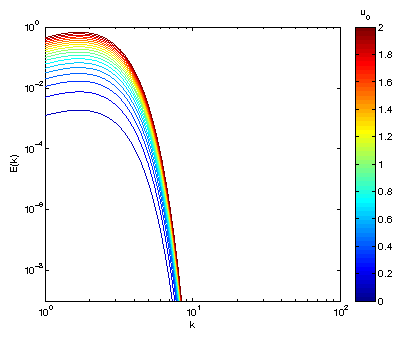
\includegraphics[width=0.48\textwidth]{Figures/eng_spr_u}
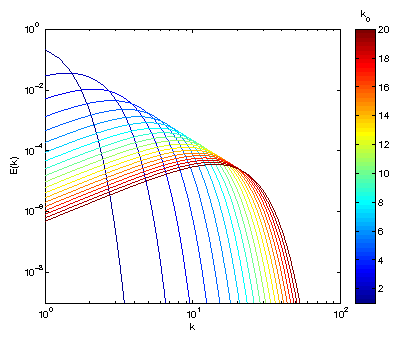
\includegraphics[width=0.48\textwidth]{Figures/eng_spr_k}
\caption{Initial energy spectrum with different parameters: left figure shows the energy spectrum with fixed $k_0 = 2.4$ while varing $u_0$ from $0m/s$ to $2m/s$, right figure shows the one with fixed $u_0 = 0.35m/s$ and varing $k$ from $1$ to $20$.\label{fig:eng_spr}}
\end{figure}

Following quantities are defined to characterize the turbulence field.  The
dissipation rate is defined as $\varepsilon=2\nu(\frac{\partial u_{i}}{\partial
x_{j}}+\frac{\partial u_{j}}{\partial x_{i}})^{2}$, $\nu$ is the kinematic
viscosity of air $1.5\times10^{-5}m^{2}s^{-1}$, and $u_{rms}$ is the root mean
square of velocity fluctuation. $\tau_{\eta}$ is the Kolmogorov time scale
defined as $(\nu/\varepsilon)^{1/2}$. $\tau_L$ is the eddy turnover time,
estimated by $L_x/u_{rms}$ where $L_x$ is the domain size.

\begin{figure}[h]\centering
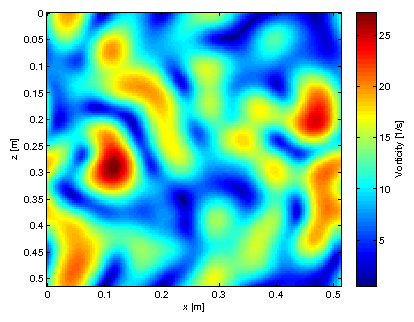
\includegraphics[width=0.48\textwidth]{Figures/vortex-0}
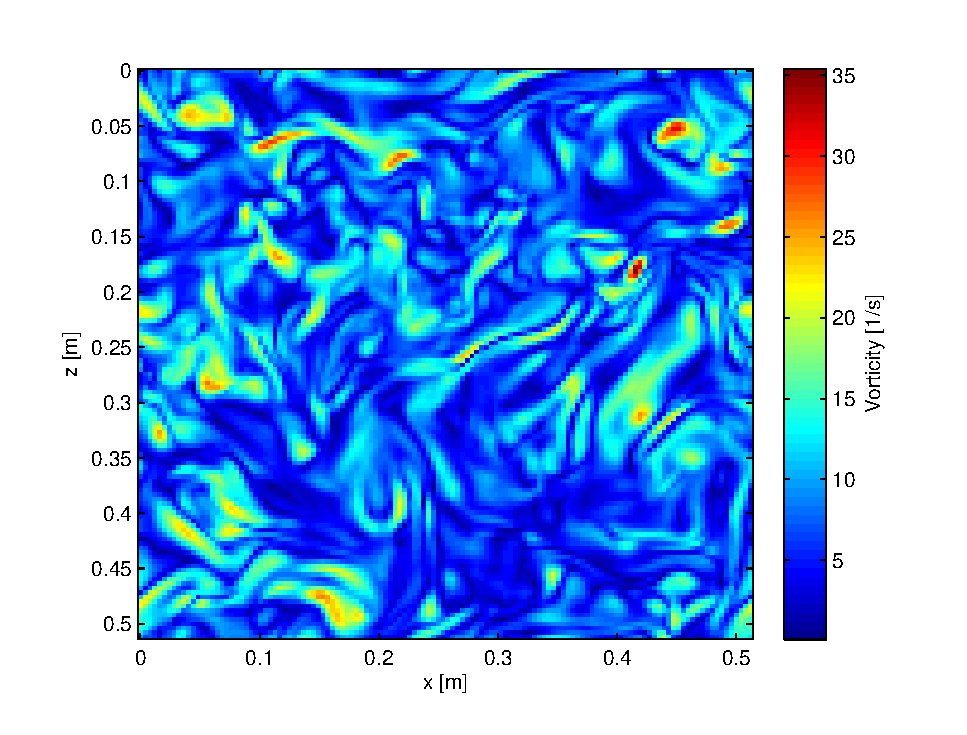
\includegraphics[width=0.48\textwidth]{Figures/vortex-1}

\caption{initial and final vorticity field ($1/s$) in x-z cross-sectional
plane for forced cases\label{fig:enstrophy}}
\end{figure}

\subsection{Initial vapor mixing ratio and temperature}
Three different initial configurations of cloudy area are used to investigate
the configuration impact. First, as in \cite{And04}, the function is defined
according to the sign of the velocity function in physics space. This
configuration is referred to as case 1 and the water vapor mixing ratio is
given by

\begin{equation}
\mbox{case 1: } q_v(\mathbf{x},t=0) = 
\left\{\begin{array}{lr}
q_v^{max}, & u(\mathbf{x}) > 0\\
q_{v,e}, & u(\mathbf{x}) \le 0
\end{array}\right.\label{case1}
\end{equation}

In \cite{Kumar11}, the author used a slab-like cloud configuration approximated with a simple discontinuous function, and is referred to as Case 2:

\begin{equation}
\mbox{case 2: } q_v(x,t=0) = 
\left\{\begin{array}{lr}
q_v^{max}, & (L-d)/2 \le x < (L+d)/2\\
q_{v,e}, & \mbox{elsewhere}
\end{array}\right.\label{case2}
\end{equation}

where $q_v^{max}$ is maximum amplitude of $q_v$, which exceeds $q_{v,s}$ by
$2\%$, and $q_{v,e} = 0.03g/kg$ is the vapor mixing ratio of the clear air. $L$
is the length of computational domain, and $d = L/2$ is the width of the cloud
slab. The simulation is terminated when droplets completely evaporate or the
field becomes nearly uniform ($std<0.0002$).

Entrainment-mixing processes can also occur near cloud tops. To mimic the
cloud-top entrainment-mixing process, herein we add a new cloud configuration
by rotating Case 2 by $90$ degree, and name it Case 3.

\begin{equation}
\mbox{case 3: } q_v(z,t=0) = 
\left\{\begin{array}{lr}
q_v^{max}, & (L-d)/2 \le z < (L+d)/2\\
q_{v,e}, & \mbox{elsewhere}
\end{array}\right.\label{case3}
\end{equation}

The temperature field is initialized by imposing the neutral buoyancy condition \cite{Kumar14}:
\begin{equation}
T(x,t = 0) = T_0 - 0.608T_0[q_v(x,t = 0) - q_{v0}]
\end{equation}
where the reference values are defined by volume averages $T_0 = \langle
T(t=0)\rangle_V$ and $q_{v0} = \langle q_v(t=0)\rangle_V$. This condition
implies that neither the vapor mixing ratio nor temperature would contribute to
the initial buoyancy. This procedure is only performed for the initial
temperature field and will completely follow \Eq{eq:Temp} afterwards.
\Fig{fig:slice_case123} illustrates the initial fields of water vapor mixing
ratio and temperature for the three cases.

\begin{figure}\centering
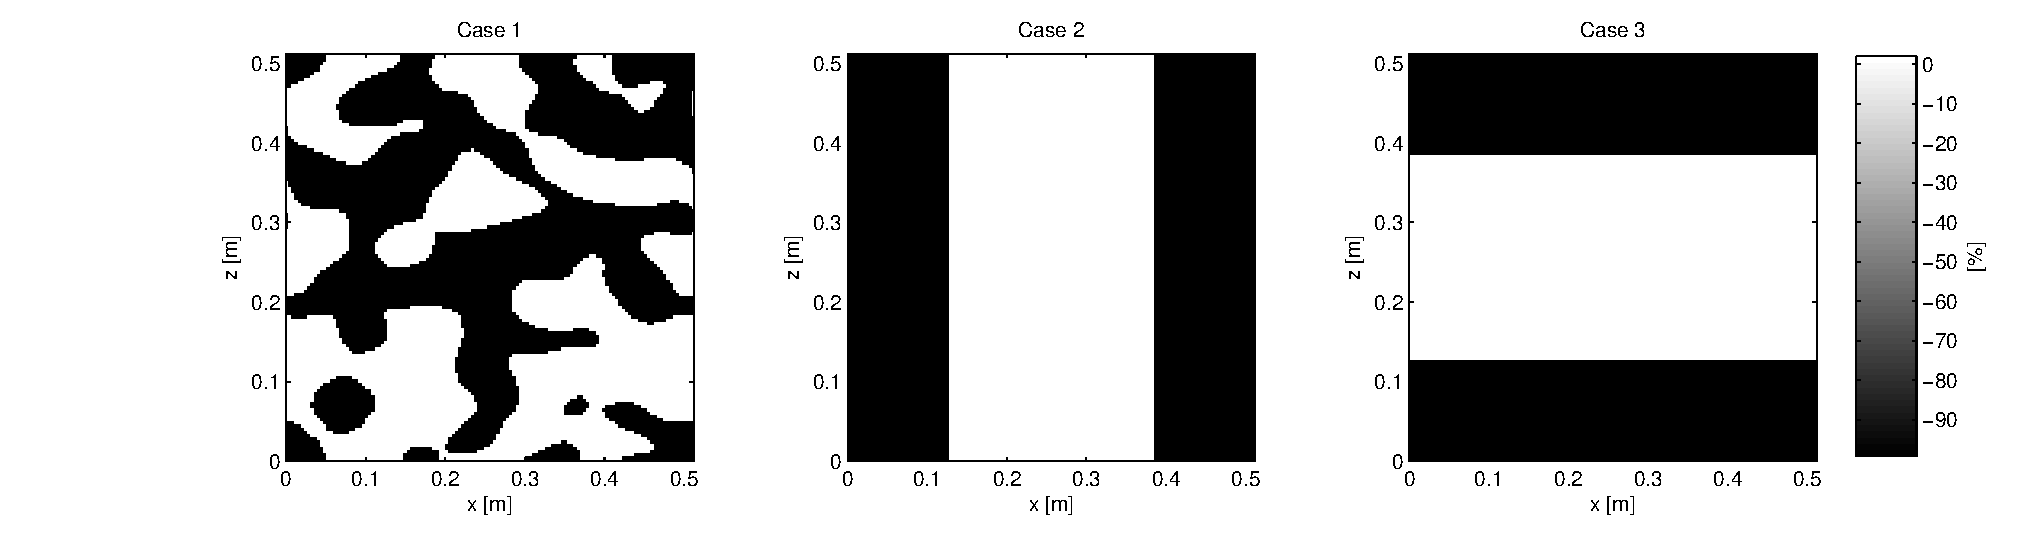
\includegraphics[width=0.8\textwidth]{Figures/supersat_case123}\\
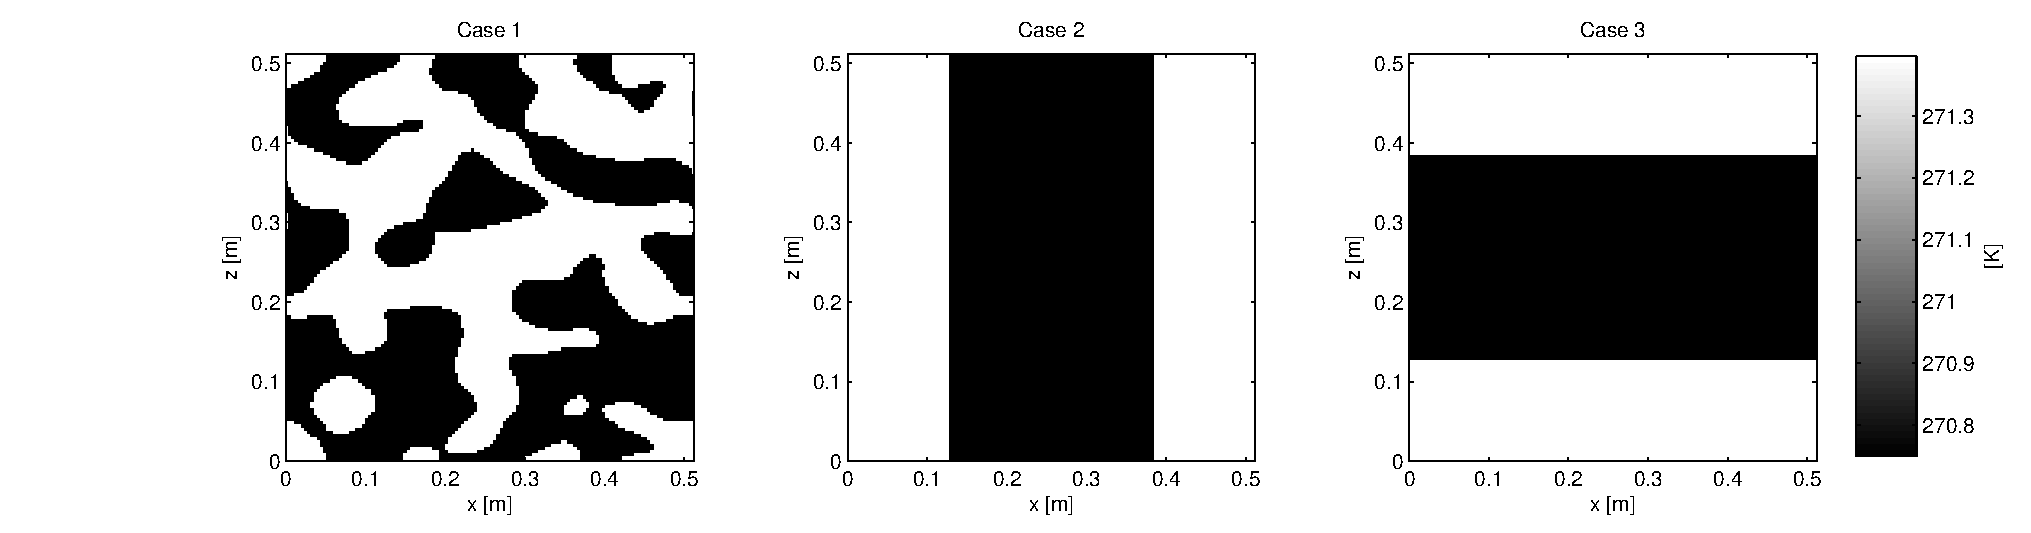
\includegraphics[width=0.8\textwidth]{Figures/temp_case123}
\caption{Cross sectional view of the initial supersaturation and temperature (K) field for different cases: case 1, 2, 3 from left to right. The cloudy part occupies about half of the computational domain.\label{fig:slice_case123}}
\end{figure}

\subsection{Initial droplets}
At beginning, a total of $10^{7}$ droplets with the same radius of $15\mu m$
are uniformly placed in the cloudy area, so as to make the droplet number
concentration about $153{cm}^{-3}$. Note that for the forced turbulence
scenario, the velocity field needs a few steps ($5$ seconds here) to relax to a
steady state. Therefore, the droplets are released to move and change their
sizes according to the physics law after this spin-up period. For the decaying
turbulence, the droplets are released at time $t = 0s$ since there is no needs
to seek for a steady state. A droplet with radius smaller than $1\mu m$ will be
immediately removed from the computational domain and will not contribute to
any statistical results.

For convenience, \Table{tb:parameters} summarizes the key quantities and initial conditions.
\begin{table}[h]
\begin{tabular}{l c c c c c}
\hline\hline
Quantity & Symbol & Value & Quantity & Symbol & Value\\
\hline
Grid points & $N$ & $256$ & Droplet radius & $R_{0}$ & $15\mu m$\\
Box length & $L$ & $0.512m$ & Environ supersat & $S_{e}$ & $-99\%$\\
Grid size & $a$ & $0.002m$ & Cloud supersat & $S_{c}$ & $2\%$\\
Viscosity & $\nu$ & $1.5\times10^{-5}m^{2}s^{-1}$ & Number density& $N_{c}$ & $153cm^{-3}$\\
Dissip rate& $\epsilon$ & $2.0\times10^{-3}m^{2}s^{-3}$ & Eddy turnover time & $\tau_{L}$ & $4.27s$\\
Dissip length& $\eta$ & $10^{-3}m$ & Evaporation time & $\tau_{evap}$ & $2.09s$\\
Dissip time& $\tau_{\eta}$ & $0.087s$ & Reaction time & $\tau_{react}$ & $4.52s$\\
\hline
\end{tabular}
\caption{Initial conditions}
\label{tb:parameters}
\end{table}

\section{Simulation Results}
\subsection{Thermodynamics}
\Fig{fig:therm_dynam} compares the temporal evolution of the turbulent kinetic
energy (a), droplets number concentration (b), standard deviation and relative
dispersion of temperature (c,d) and the same for water vapor mixing ratio
(e,f).

In panel (a), the turbulent kinetic energy (TKE) of the forced cases F1, F2 and
F3 remains on average after a short relaxation at the initial time. However, it
is interesting to observe a transient growth in the decaying cases before
continuing to decay to zero. We interpret this growth as the results of
buoyancy effect, which is caused by the deviation of temperature and vapor
mixing ratio to the reference value according to \Eq{eq:source_term}. In
details, case D1 could be regarded as the intermediate stage of mixing process
in D2 or D3, therefore this deviation quickly disappear and show no growth in
the figure. As for D2, the mixing only happens at the interface between cloudy
and clear air, thus it takes much longer to damp the transient growth. The
mixing in case D3 is accelerated by sedimentation effect, making it a little
faster than D2.

The droplets number concentration for different cases are displayed in panel
(b). All cases have the same equilibrium state with a zero liquid water
content, i.e., all droplets eventually evaporate. The rate at which droplets
evaporate is higher for the forced turbulence than the decaying turbulence
except D1. In D1 all the droplets quickly be exposed to the same environment
and begin to evaporate, leading to its number concentration curve to be similar
as the forced cases.

Panel (c) and (d) show the standard deviation and relative dispersion of
temperature field. In spite of similar configuration with D2, case D3 has a
stronger growth in amplitude. We interpret this phenomenon as sedimentation
effect, indicating that the droplet movements are accelerated in the vertical
direction by gravity. Most of the droplets have a chance to enter into the
clear air and evaporate at an early stage. This evaporation process absorb
latent heat from the environment thus strongly making the temperature field
deviate from the mean value. However, this difference becomes smaller in the
forced turbulence since the motion of particles is predominantly controlled by
the external forcing, which are the same for F1, F2 and F3.

\ref{fig:therm_dynam} (e) and (f) show the standard deviation and relative
dispersion of vapor mixing ratio, respectively. In these figures, we cannot
observe any transient growth as shown for temperature field. This result is
consistent with \cite{Kumar14}. Notice that the vapor mixing ratio in the clear
air is much lower than in the cloudy air. The droplets entering into the clear
area will quickly turn into vapor while the droplets staying in the cloudy area
continue to condensate. This phase transition process reduce the difference of
vapor mixing ratio between clear air and cloudy air, thus the transient growth
of the deviation can hardly be observed.

\begin{figure}\centering 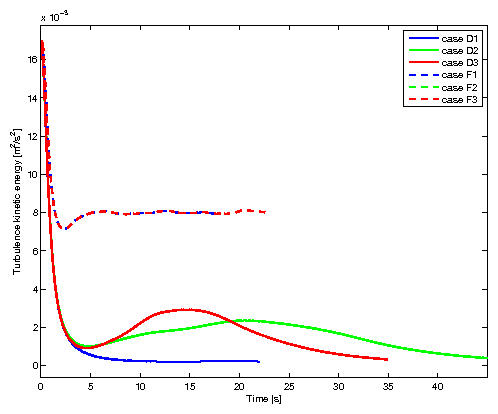
\includegraphics[width=0.48\textwidth]{Figures/tke}
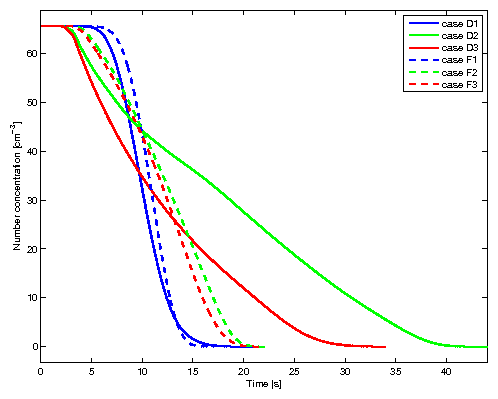
\includegraphics[width=0.48\textwidth]{Figures/num_con}\\
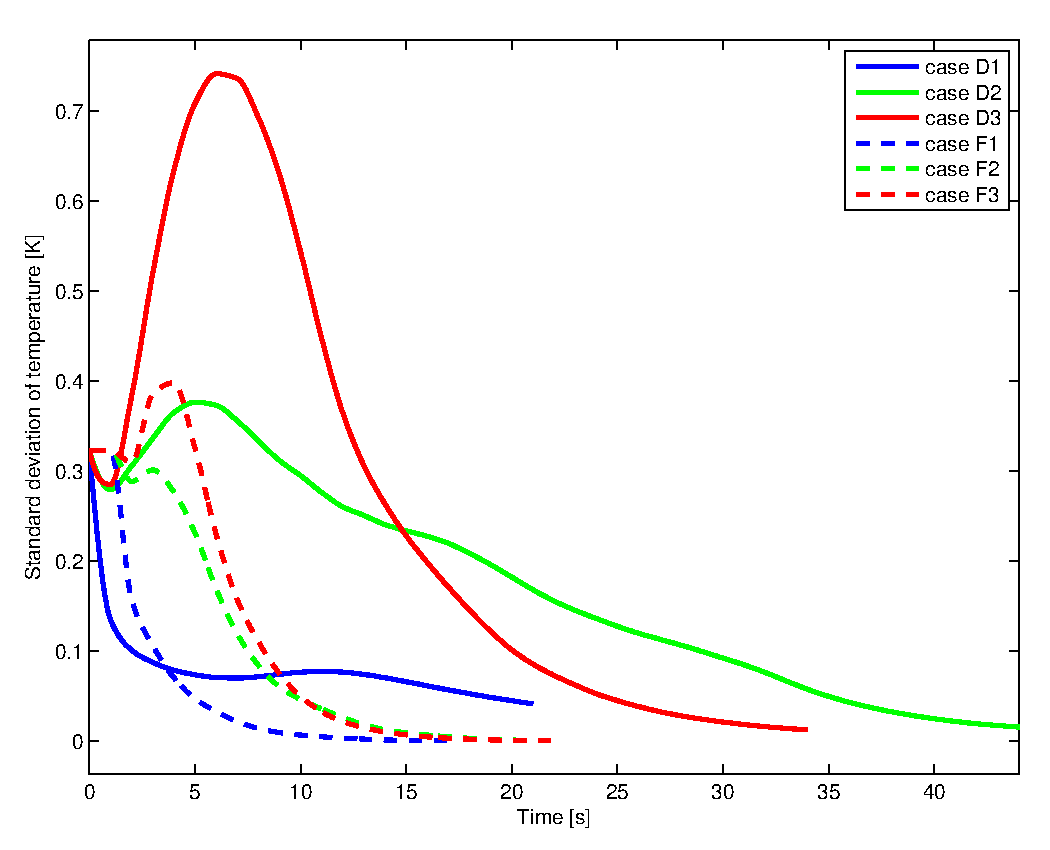
\includegraphics[width=0.48\textwidth]{Figures/temp_std}
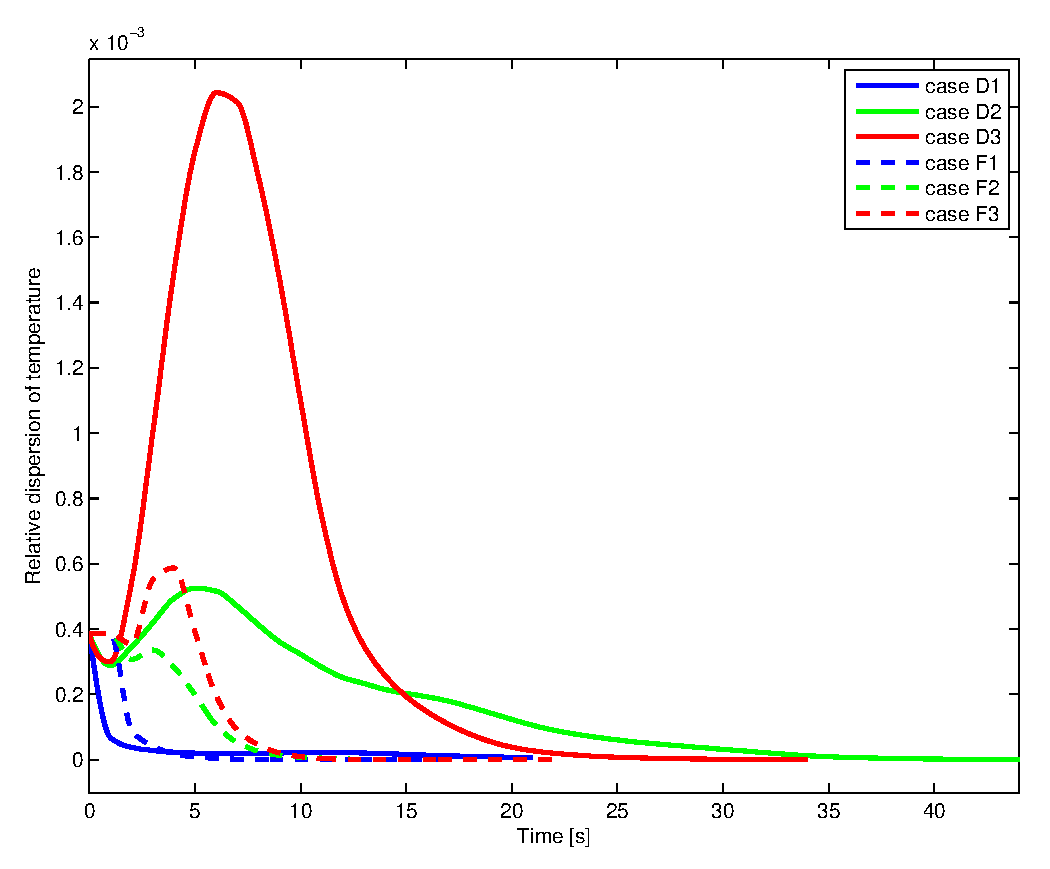
\includegraphics[width=0.48\textwidth]{Figures/temp_dsp}\\
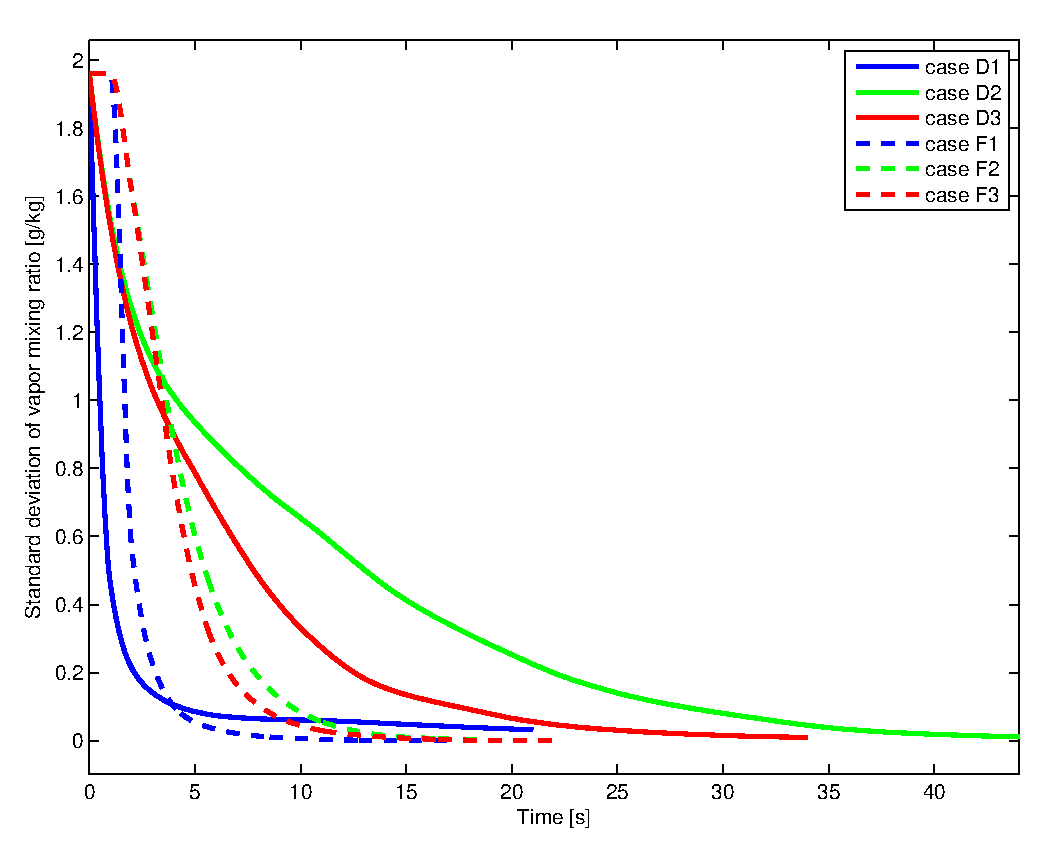
\includegraphics[width=0.48\textwidth]{Figures/vapor_std}
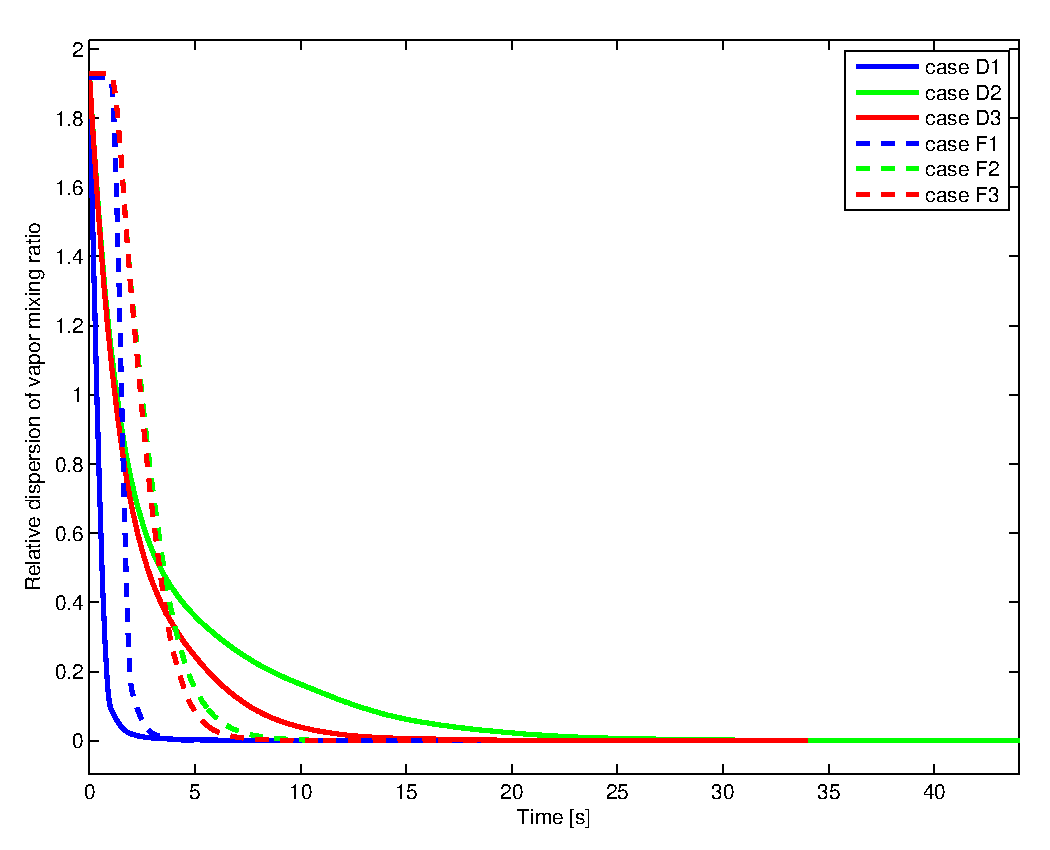
\includegraphics[width=0.48\textwidth]{Figures/vapor_dsp}
\caption{Thermodynamics of three cases, from left to right, up to bottom, are
turbulence kinetic energy (a), droplets number concentration (b), standard
deviation (c), relative dispersion (d) of temperature field and the same for
the vapor mixing ratio (e,f).\label{fig:therm_dynam}} \end{figure}

\subsection{Microphysics}
The droplet size distributions for case 1, 2 ,3 in both decaying and forced
turbulence are displayed in \Fig{fig:rad_distri}. At the initial stage, some
droplets enter into the clear air and expand their size distribution. As mixing
going on, since the environment is unsaturated and homogeneous, the
distribution gradually shift to small sizes until all droplets completely
evaporate or the background environment becomes saturated.  An important
observation is that case D1, D2 and D3 are quite different in both reaction
time and size distribution. However, by adding the external force, these
difference almost disappear. This demonstrates that the role of buoyancy effect
is overwhelmed by the external forcing and the differences in the decaying
cases are caused by the buoyancy term in \Eq{eq:source_term}. In specific, the
buoyancy plays as a source of kinetic energy, so as to influence the motion of
the fluid field.  

\begin{figure}[h]\centering
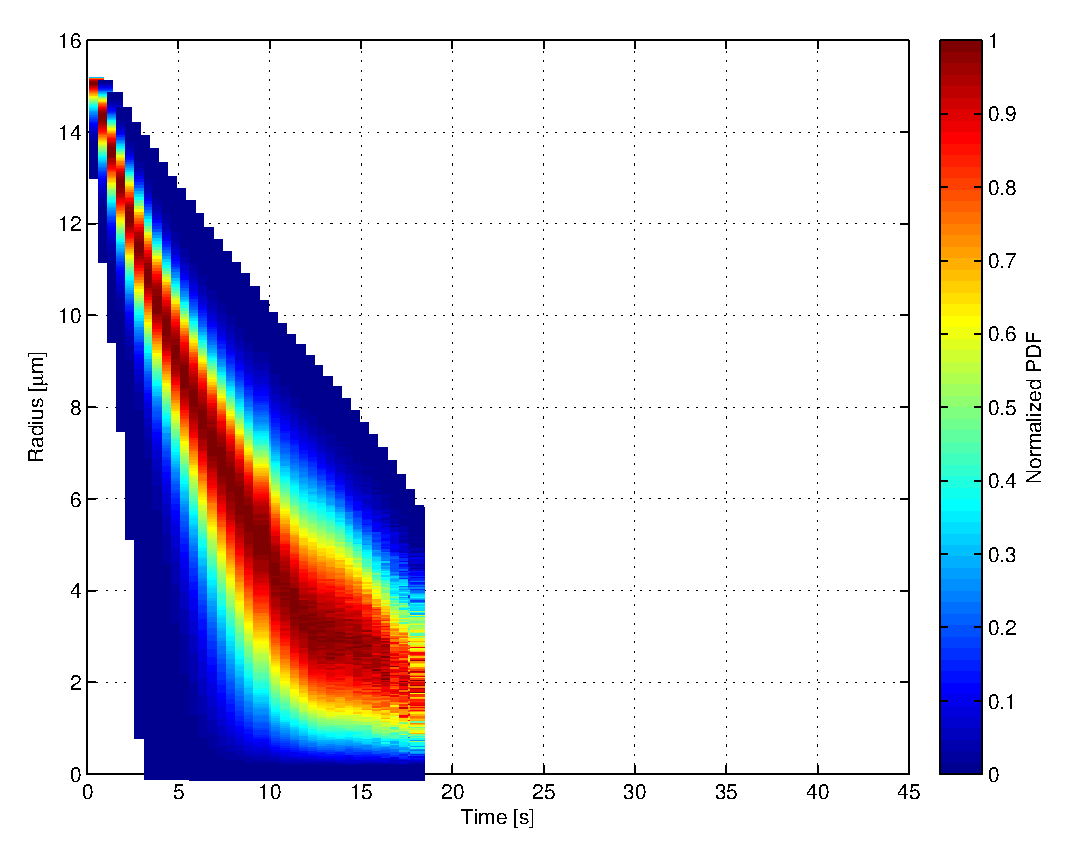
\includegraphics[width=0.48\textwidth]{Figures/pdf_radius_d1}
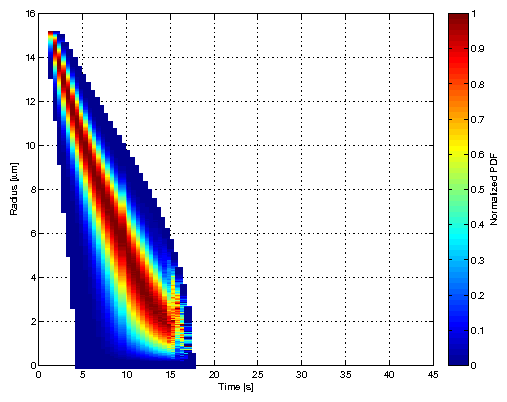
\includegraphics[width=0.48\textwidth]{Figures/pdf_radius_f1}\\
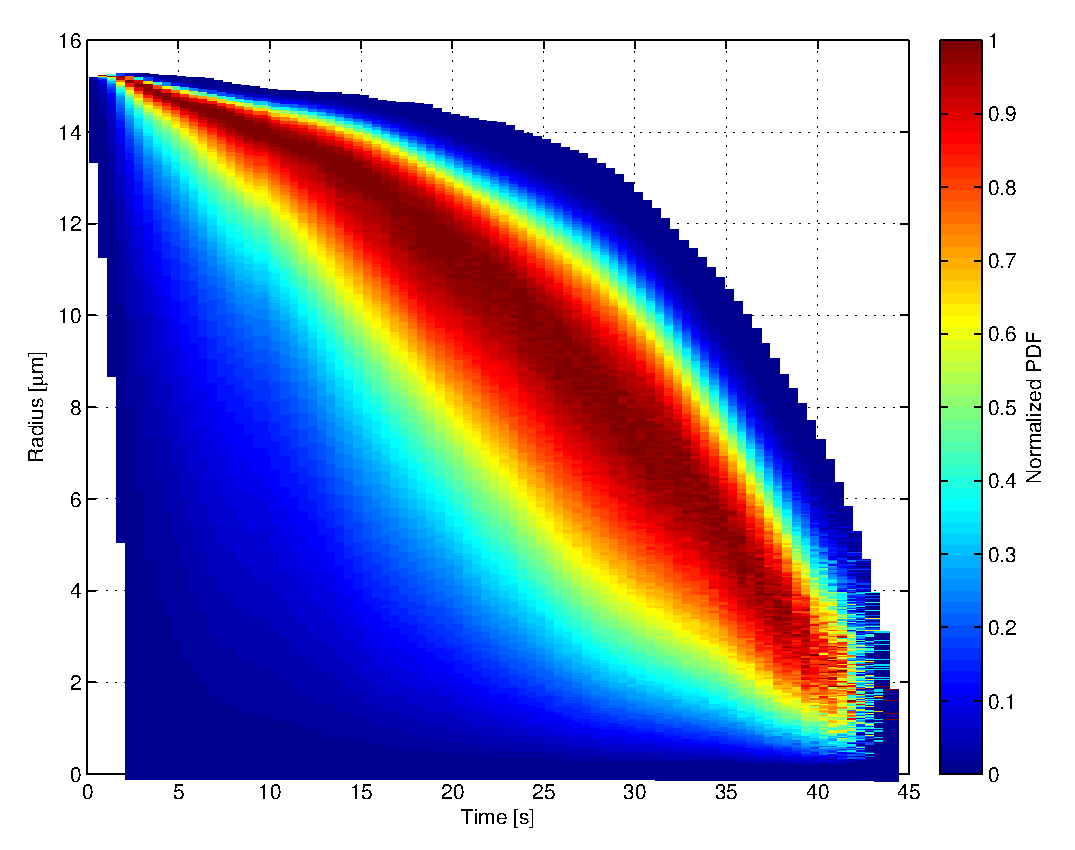
\includegraphics[width=0.48\textwidth]{Figures/pdf_radius_d2}
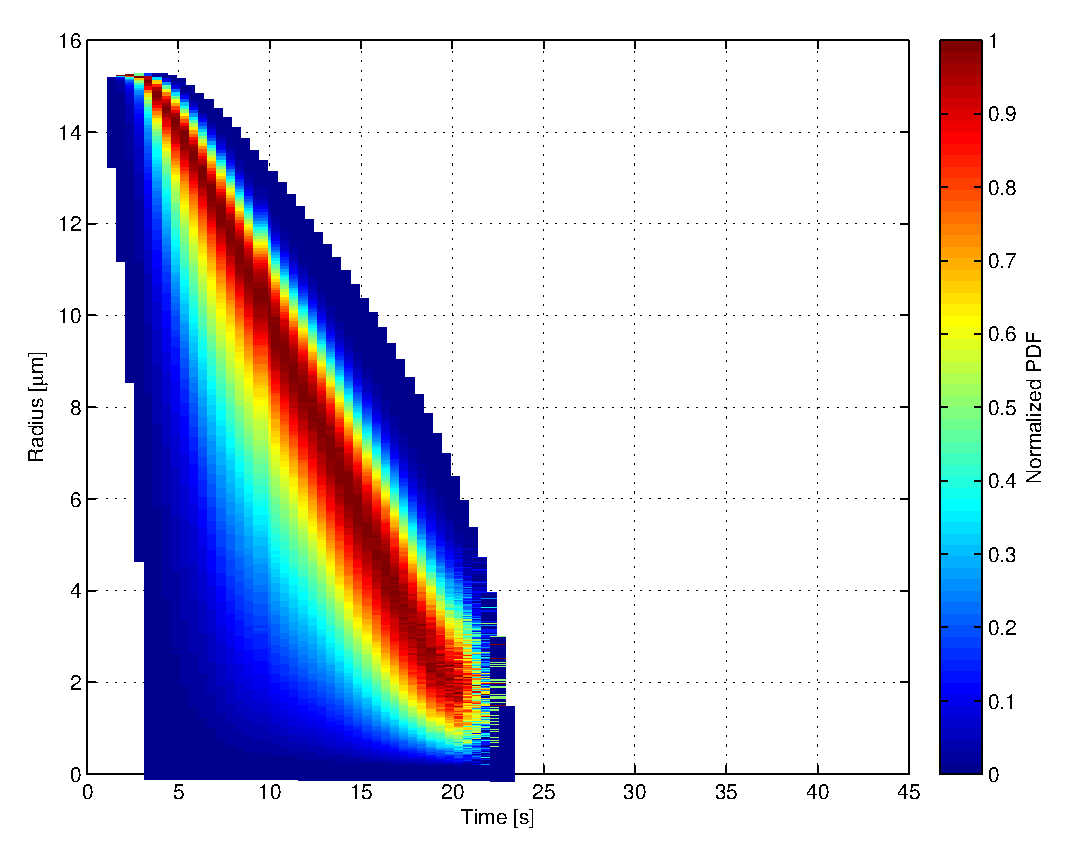
\includegraphics[width=0.48\textwidth]{Figures/pdf_radius_f2}\\
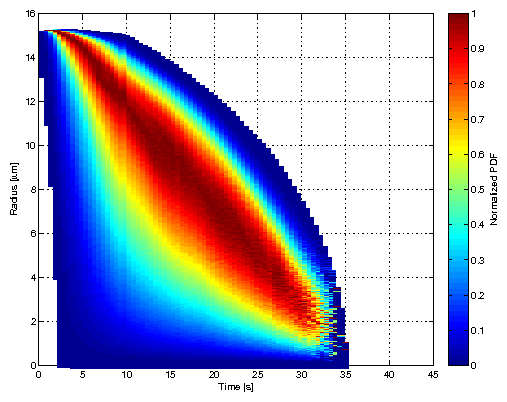
\includegraphics[width=0.48\textwidth]{Figures/pdf_radius_d3}
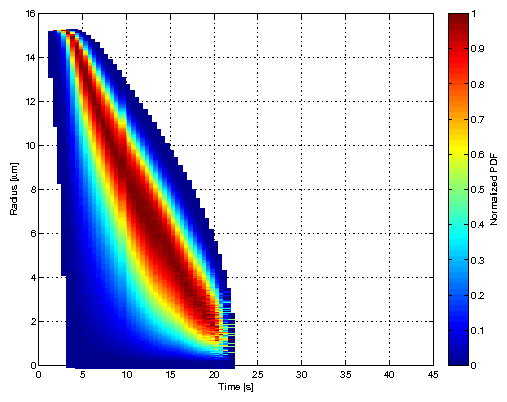
\includegraphics[width=0.48\textwidth]{Figures/pdf_radius_f3}
\caption{Evolution of radius distribution for decaying turbulence (left column)
and forced turbulence (right column). From up to bottom are case 1, case 2 and
case 3 respectively.}\label{fig:rad_distri} \end{figure}

The distribution of supersaturation in \Fig{fig:supersat_distri} also clearly
reflects the mixing process. In the initial period, most of the droplets stay
in the cloud filaments, and thus has narrow probability density distribution
(PDF). After some droplets entering into the clear air, the spectrum
immediately expands with low probability density. This stage could be observed
in D2 and D3, but extremely short for the rest cases. As mixing proceeds, the
environment becomes much more homogeneous, that is most droplets stay in a
similar environment. Finally, the environment becomes well-mixed, droplets
completely evaporate and all the cases reach the same state.

\begin{figure}[h]\centering
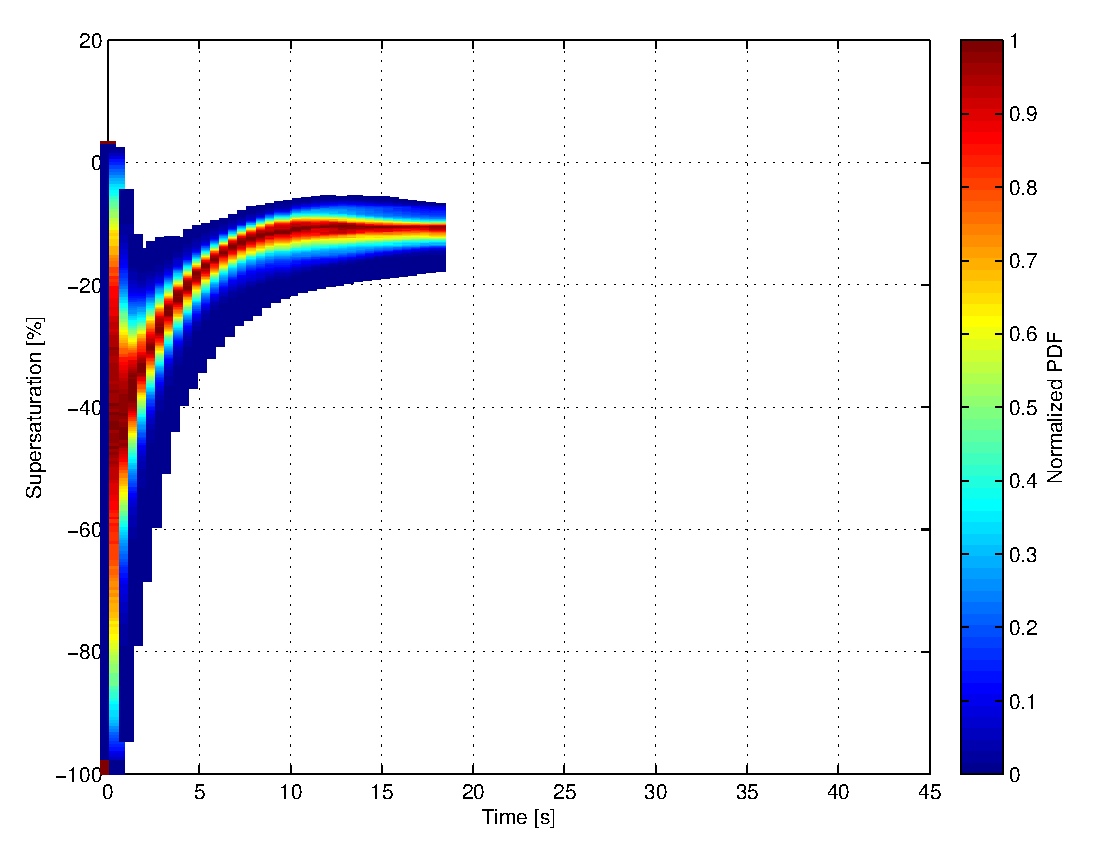
\includegraphics[width=0.48\textwidth]{Figures/pdf_supersat_d1}
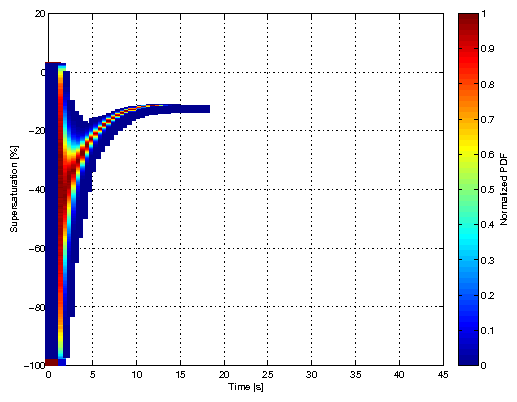
\includegraphics[width=0.48\textwidth]{Figures/pdf_supersat_f1}\\
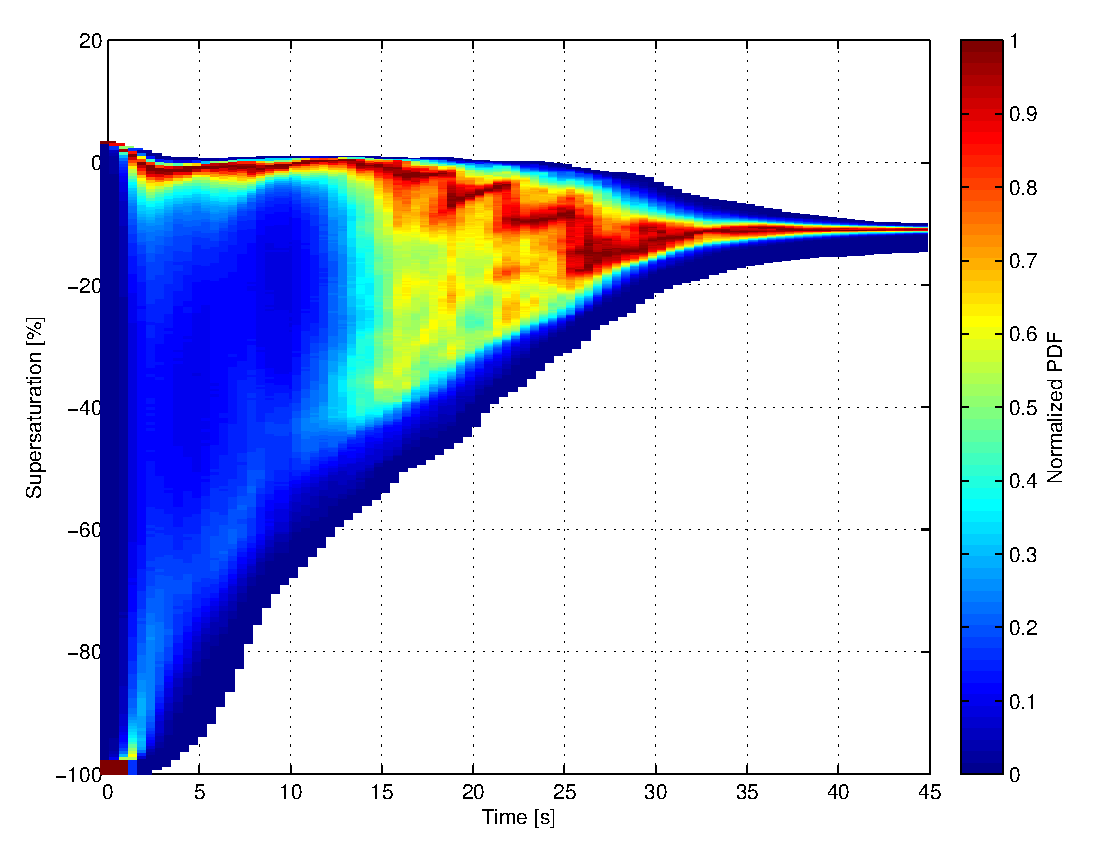
\includegraphics[width=0.48\textwidth]{Figures/pdf_supersat_d2}
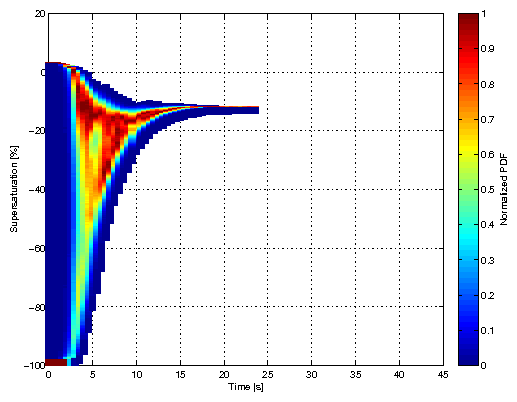
\includegraphics[width=0.48\textwidth]{Figures/pdf_supersat_f2}\\
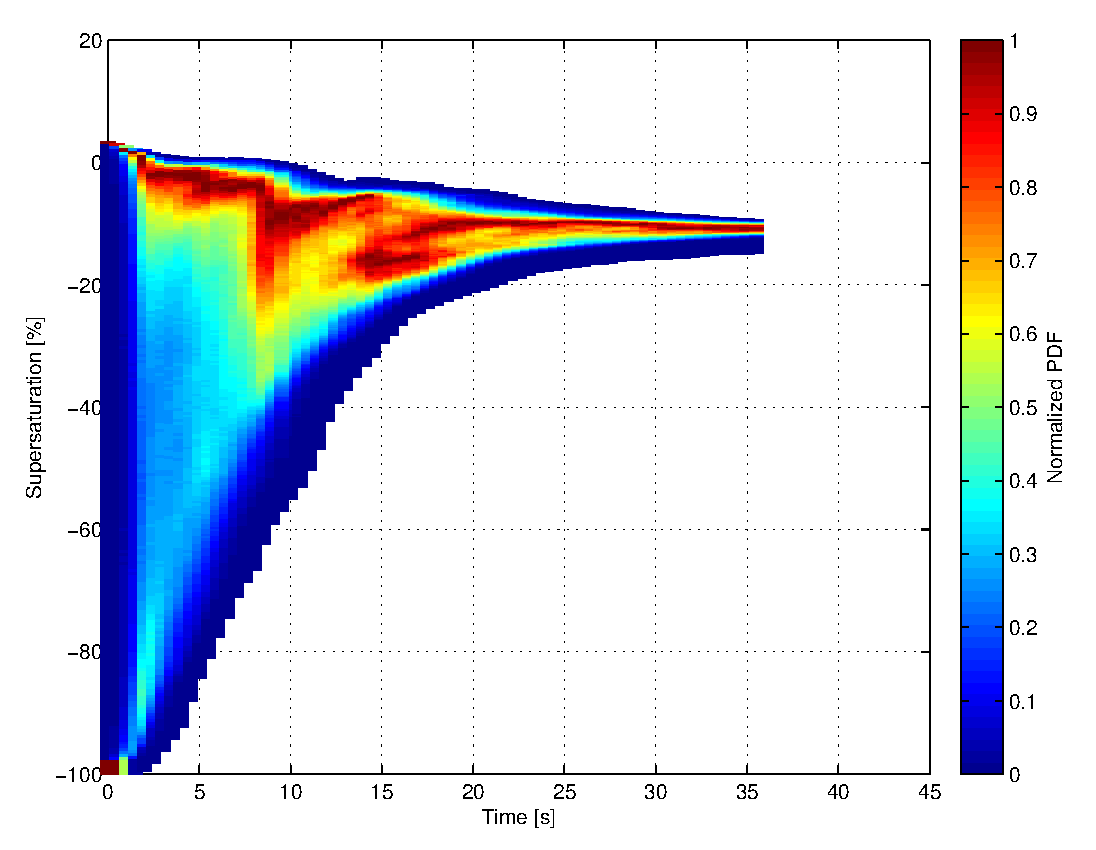
\includegraphics[width=0.48\textwidth]{Figures/pdf_supersat_d3}
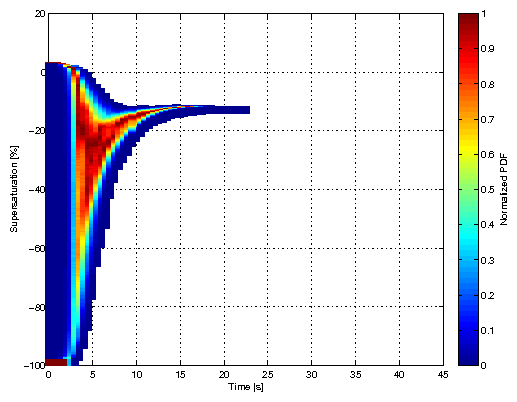
\includegraphics[width=0.48\textwidth]{Figures/pdf_supersat_f3}
\caption{Evolution of supersaturation distribution for decaying turbulence
(left column) and forced turbulence (right column). From up to bottom are case
1, case 2 and case 3 respectively. In conclusion, the shape of the cloud
filament has no influence on the final state after the mixing but will affect
the intermediate process. The shape also has little impact on the mixing
process for forced turbulence, while can not be completely ignored in the
decaying cases. The results suggest that the initial shape of cloud filaments
should be considered as an important factor when studying mixing scenario
without external forcing.}\label{fig:supersat_distri} \end{figure}

\subsection{Mixing scenario}\label{mixing_processes} Depending on the mixing
scenario (the homogeneity of mixing), the droplets evolve in quite different
ways. In the extremely homogeneous mixing scenario, droplet concentration does
not change while liquid water mixing ratio and thus the mean radius decreases.
In the extremely inhomogeneous mixing scenario, some droplets in the cloud
completely evaporate, reducing droplet number concentration and liquid water
mixing ratio while keeping mean radius roughly unchanged. The mixing of clear
and cloudy air is often quantified by the Damkohler number:

\begin{equation}
Da=\frac{\tau_{mix}}{\tau_{react}}\label{eq:DaNumber}
\end{equation}

where $\tau_{mix}$ is the turbulent mixing time scale for an eddy of size $l_E$ given by:

\begin{equation}
\tau_{mix}=(\frac{l_E^{2}}{\varepsilon})^{1/3}\label{eq:Tmix}
\end{equation}

The evaporation time $\tau_{react}$ defined as either the time when the
droplets have completely evaporated or the time at which the averaged
supersaturation $S > -0.005$.

In general, $Da\ll1$ corresponds to the homogeneous mixing while $Da\gg1$ is
the inhomogeneous one. Ambient clouds often have $Da$ between these two limits.

In spite of popularity, this approach has a shortcoming: the value of $l_E$
used in (\ref{eq:Tmix}) is ambiguous. To overcome this difficulty,
\cite{Lehmann09} introduced the concept of transition length $l^{*}$, at which
the mixing transits from inhomogeneous to homogeneous:

\begin{equation}
l^{*}=\varepsilon^{1/2}\tau_{react}^{3/2}\label{eq:TransL}
\end{equation}

With transition length $l^{*}$, a dimensionless number called transition scale
number was introduced in \cite{Chunsong13} and defined as the ratio of $l^{*}$
and Kolmogorov length scale $\eta$:

\begin{equation}
N_{L}=\frac{l^{*}}{\eta}\label{eq:NL}
\end{equation}

The $\tau_{react}$ can also be computed by solving the following ordinary
differential equation with volume mean radius and mean supersaturation as the
initial condition:

\begin{equation}
\frac{dR_{m}}{dt}=K\frac{S}{R_{m}}\label{eq:DiffR}
\end{equation}

\begin{equation}
\frac{dS}{dt}=-BR_{m}S\label{eq:DiffSuper}
\end{equation}
where $B$ is a function of pressure and temperature:
\begin{equation}
B = 
\frac{4\pi N\rho_L[\frac{R_dT}{\varepsilon e_s(T)} + \frac{\varepsilon L^2_h}{pTc_p}]} 
{(\frac{L_h}{R_vT}-1)\frac{L_h\rho_L}{KT} + \frac{\rho_L R_v T}{De_s(T)}}
\end{equation}

where $L_h$ is latent heat, $R_v$ is individual gas constant for water vapor,
$T$ is air temperature, $\rho_L$ is density of liquid water, $K$ is coefficient
of thermal conductivity of air, $D$ is coefficient of diffusion of water vapor
in air, $e_s(T)$ is saturation vapor pressure over a plane water surface at
temperature $T$, $N$ is number concentration of droplets, $R_d$ is individual
gas constant for dry air, $\varepsilon = R'/R_v$, $p$ is air pressure, and
$c_p$ is specific heat with pressure held constant (\cite{Lu2011}).

To characterize the microphysical properties of the mixing, the $\langle
r^3\rangle -N_d$ diagram (volume mean radius versus number density) was
introduced in \cite{Burnet07} and has been widely applied to study the
homogeneous/inhomogeneous entrainment-mixing process. Taking advantage of
$\langle r^3\rangle -N_d$ diagram, one can predict the extremely homogeneous
mixing line with different initial liquid water content and vapor mixing ratio
(\cite{Lehmann09,Kumar14}).

Similar to \cite{Kumar14}'s idea, the computational domain is divided into $64$
equal-sized sample boxes. We keep tracking the volume mean radius and number
concentration at each time step for each sample box and scale them by the
adiabatic values, which are the values in the cloudy area. The mixing diagrams
for different cases are displayed in \Fig{fig:mixing_diagram}. In the mixing
diagram, each curve indicated by different colors represents the temporal
history of $R_v^3/R_a^3$ and $N_d/N_a$ in each sample box; the homogeneous
mixing line (red dotted) and inhomogeneous mixing line (black dotted) are
plotted in the diagram as reference (see \cite{Burnet07} for how to plot
homogeneous mixing line).

In the top panel, the mixing diagram of D1 and F1 do not start from the $(1,1)$
point since the initial droplets in a sample box have already been diluted and
their number concentration are much less than the adiabatic value. The droplets
number concentration remains nearly unchanged until some droplets completely
evaporate. As claimed in \cite{And04}, this configuration excludes the dilution
process and can only be used to simulate the final stage of the entrainment and
mixing process. The difference between forced turbulence and decaying
turbulence is not obvious, except a wider range of variability in the shape of
the mixing trajectories for the decaying turbulence D1, since the forced
turbulence will foster the mixing procedure, resulting in similar states in
different sample boxes.

In the middle panel, the mixing diagram shows the mixing curves for case D2 and
F2. These cases have the same configurations with \cite{Kumar14}. However, a
sharp initial profile of vapor mixing ratio was used in our simulation. This
results in an unsaturated vapor mixing ratio at final state, leading to
completely evaporation of the droplets. The phenomenon of inhomogeneous offset
described by \cite{Kumar14} could also be observed in the figures: the mixing
trajectories tend to shift to smaller values of $N_d/N_{d,a}$. This
inhomogeneous offset is almost due to the initial dilution process, in which
the droplets number concentration in the sample boxes is diluted while the
droplets mean radius in the sample box doesn't change too much. As mixing
proceeds, the turbulent time scale in the decaying case continues to increase
while the time scale for the forced turbulence remains unchanged. Therefore,
the inhomogeneous mixing is more likely to happen in case D2, leading to a
strong deviation from the homogeneous mixing line.

A similar conclusion can be obtained in the bottom panel for case D3 and F3.
However, it is interesting to observe two groups in the mixing trajectories. We
interpret this divergence by considering the following facts. According to our
way of selecting sample boxes, the cloud slab will be divided into two groups:
the upper layer (red) and the lower layer (blue). On one hand, due to the
sedimentation effect, a part of the droplets will escape from the upper layer
and enter into the lower layer, thus making the number concentration of upper
level sample boxes decreased and their volume mean radius unchanged. On the
other hand, the evaporating droplets below the lower layer may reentering into
the lower sample boxes by the turbulent mixing, leading to reduced volume mean
radius and slowly decreasing number concentration.

The quantities mentioned at the beginning of this section can be used as good
predictors of the mixing scenario. As shown in \Table{tb:parameters}, the eddy
turnover time $\tau_L = 4.27s$, evaporation time scale $\tau_{evap} = 2.09s$
and reaction time scale $\tau_{react} = 4.52s$. Defining a Damkohler number
based on $\tau_{evap}$ gives $Da_{L,evap} = 2.04$, which is significantly
greater than unity and seems to favor a strong inhomogeneous mixing in the
inertial range. However, during mixing, the evaporation of droplets gradually
saturate surrounding vapor and therefore the chemical reaction will spend
longer time to complete. This implies that the assumption of constant
supersaturation for the $\tau_{evap}$ is not strictly correct.  As opposed to
$\tau_{evap}$, the definition of $\tau_{react}$ based on \Eq{eq:DiffR} and
\Eq{eq:DiffSuper} considers the interactions between radius $R$ and
supersaturation $S$ and therefore should be more suitable to predict the
thermodynamic time scale. Defining the Damkohler number based on $\tau_{react}$
results in $Da_{L,react} = 0.94$, slightly lower than unity and hence yields an
intermediate state between the homogeneous and inhomogeneous mixing. In fact,
the transition length scale is equal to $l^{*} = 0.426m$, defining the length
scale within the inertial range at which $Da = 1$. This $l^*$ is somewhat
smaller than the domain size $0.512m$ but $400$ times greater than the
Kolmogorov length scale. As the turbulence eddies evolve from the energy
containing length $L_x$, through $l^*$, and down to the smallest length scale
$\eta$, the mixing scenario quickly expands from inhomogeneous to homogeneous
mixing. The side length of the sample boxes $0.512m/4 = 0.128 m$ is
significantly smaller than $l^* = 0.426m$, thus an extreme homogeneous mixing
is most possible to be observed. However, from \Fig{fig:mixing_diagram}, the
relationship between the mixing trajectory and mixing scenario is not obvious.
The mixing trajectories do not have to follow the homogeneous mixing line
although the mixing scenario is expected to be homogeneous. Moreover, the
behaviors of the mixing trajectories for different cases differ from each other
even if they have the same liquid water content and initial turbulence
settings. In conclusion, the behaviors of the mixing trajectories are not only
determined by the relative time scale or Damkohler number but also by the
distribution of the cloud water content.

\begin{figure}\centering
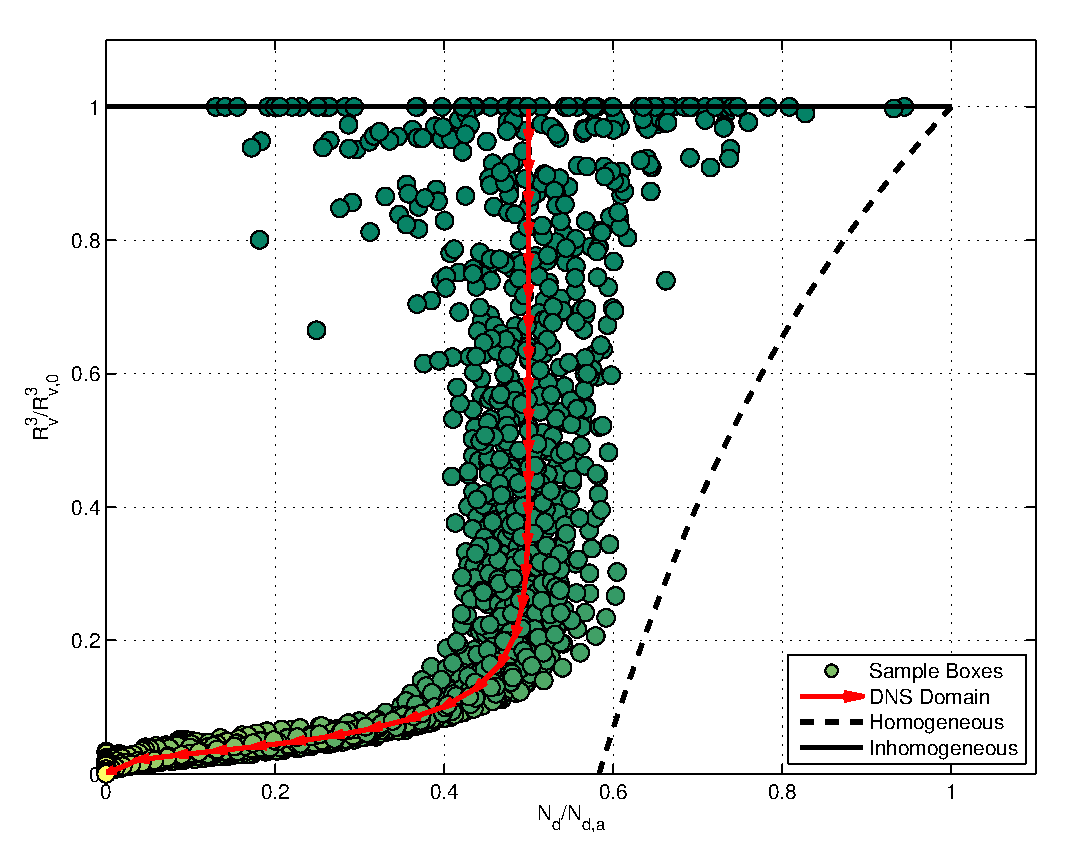
\includegraphics[width=0.48\textwidth]{Figures/mixing_cased1}
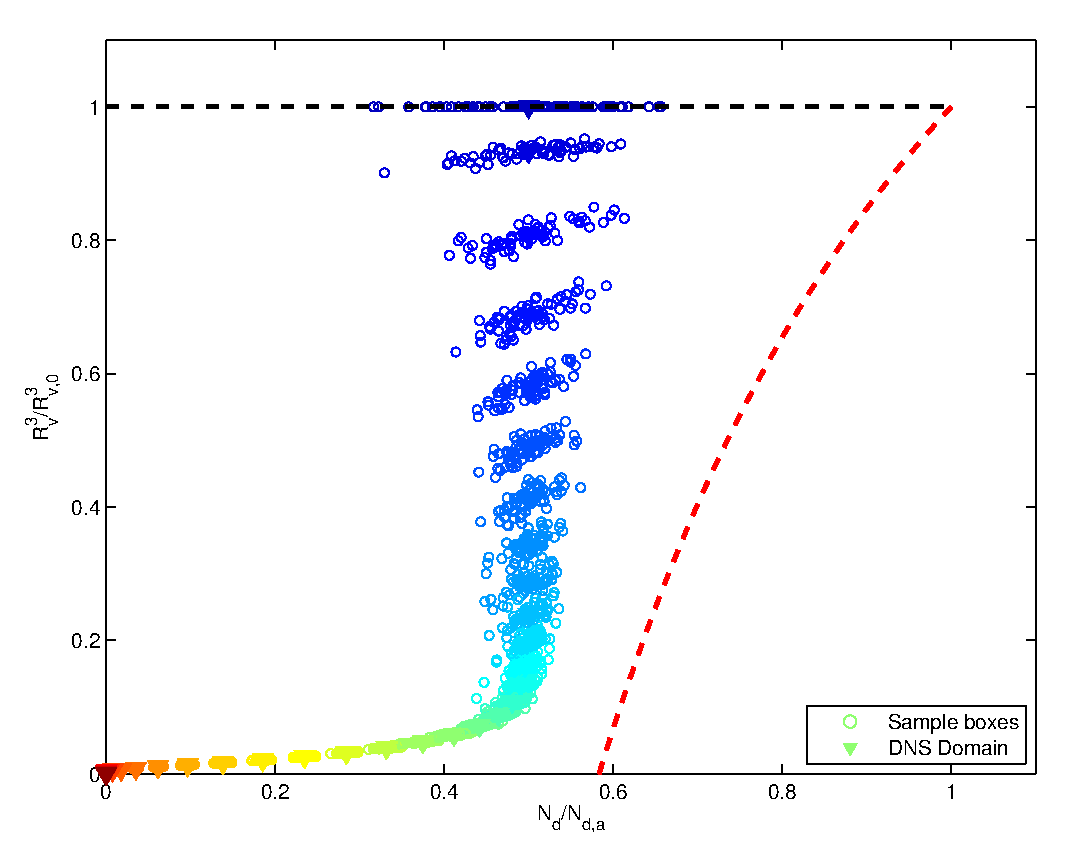
\includegraphics[width=0.48\textwidth]{Figures/mixing_casef1}\\
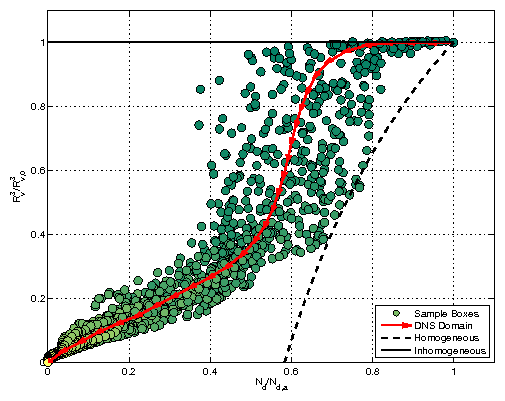
\includegraphics[width=0.48\textwidth]{Figures/mixing_cased2}
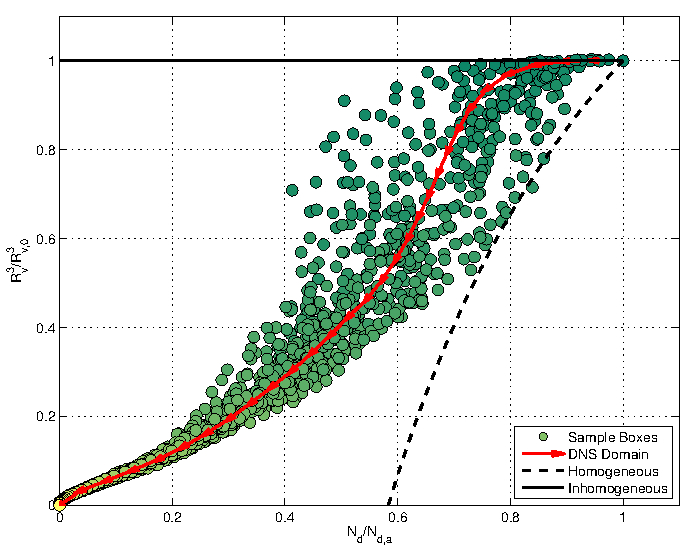
\includegraphics[width=0.48\textwidth]{Figures/mixing_casef2}\\
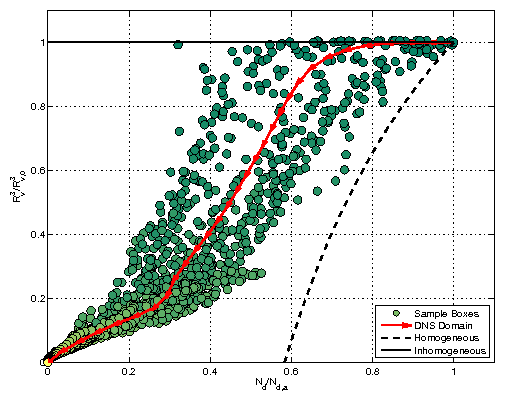
\includegraphics[width=0.48\textwidth]{Figures/mixing_cased3}
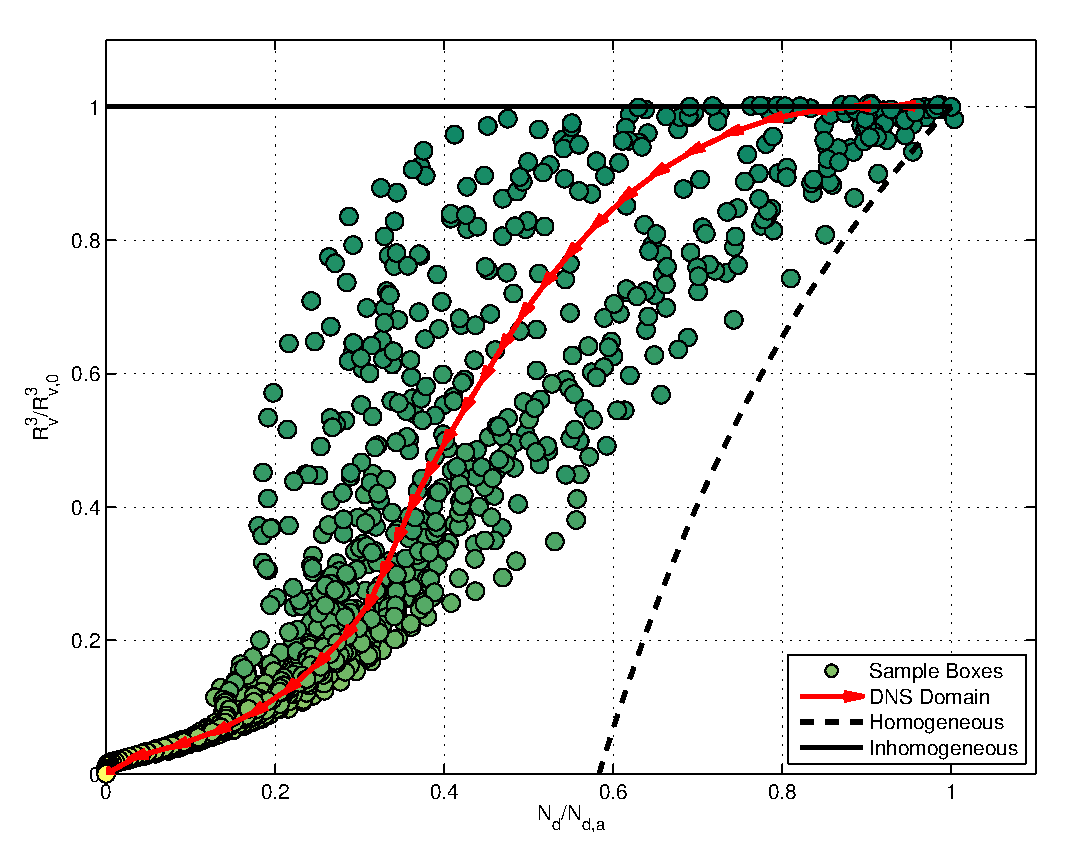
\includegraphics[width=0.48\textwidth]{Figures/mixing_casef3}
\caption{Mixing diagram for case D1, D2, D3, F1, F2 and F3. Mean cubic radius
and mixing fraction have been calculated in 64 equal-sized samples boxes. The
circle represent the time trajectories of $R_v^3/R_{v,0}^3$ and $N_d/N_{d,a}$
in different sample boxes and the triangles represent the same in the entire
domain. Color indicates the time for each record. Only the boxes with non-zero
particles at the initial time are considered. \label{fig:mixing_diagram}}
\end{figure}

\subsection{Effects of sedimentation on preferential concentration}
Clustering of inertial particles has been extensively studied via both
experiments and numerical simulations \cite{Sundaram97, Reade2000}, but the
sedimentation effects on the clustering are poorly understood. In this section,
a series of numerical test are performed by gradually increasing the gravity
force. Since we are only interested on the functional relationship between
clustering index and gravity, the particles are not allowed to evaporate or
condensate during the simulation, thus keeping their sizes unchanged.  The
clustering index calculated with \cite{Vaillancourt02}

\begin{equation}
C_L = \hat{V}_L(n)/V_L(n)-1
\label{eq:cluster_index}
\end{equation}

where $\hat{V}_L(n)$ is the measured variance of the droplets number
concentration and $V_L(n)$ is the Poisson variance equal to the mean droplet
number concentration. The droplets are uniformly placed in the domain at
initial time, thus their number concentration will follow the Poisson point
distribution.

From the history of the clustering index in \Fig{fig:gravity_cluster}, one can
tell that the clustering indexes increase at the beginning stage due to the
strong turbulence fluctuation and then decrease as the turbulence decaying. The
forced turbulence differs from the decaying case by remaining on average of
clustering index in the latter stage of the simulation. The result suggests
that gravity weakens the preferential concentration. This phenomenon can also
be visualized in \Fig{fig:sed_gravity} by plotting the clustering index as a
function of the gravity at the final step.

Preferential concentration can also be measured with Pearson correlation
coefficient between droplet number concentration and vorticity magnitude.
\Fig{fig:correlation} shows the correlation coefficients of four cases,
decaying or force turbulence with or without considering sedimentation as a
function of time. All the cases show negative correlations, which agrees with
that particles tend to accumulate within the low vorticity area of turbulence
field. Two nondimensional numbers are useful for understanding the mechanism of
preferential concentration. One is the Stokes number, which measures the
relative time scale of particle and turbulence flow:
\begin{equation}
S_t = \tau_p/\tau_{\eta}
\end{equation}
where $\tau_p = 2\rho_wR^2/9\mu$ is the particle response time and
$\tau_{\eta}$ is the Kolmogorov time scale.

Previous studies \cite{grabowski1999comments,vaillancourt2000review} have shown
that maximum preferential concentration occurs at $S_t \sim 1$. For sedimenting
particles, another useful nondimensional number is based on the terminal
velocity of the particles:
\begin{equation}
S_v = v_T/v_{\eta}
\end{equation}
where $v_T = \tau_p g$ is the terminal velocity and $v_{\eta}$ is the
Kolmogorov velocity scale. The droplets have no time to interact with the
eddies when $S_v \gg 1$ and sedimentation can be neglected when $S_v \ll 1$,
thus $S_v \sim 1$ represents the case that sedimentation effects should not be
ignored.

In our simulation, the initial condition gives $\tau_p = 0.0028 s$, $\tau_\eta
= 0.087s$ and $S_t = 0.032$; $v_T = 0.027 m/s$, $v_{\eta} = 0.011 m/s$ and $S_v
= 2.45$. The fact of $S_t \ll 1$ tells that the particle motion will almost
follow the turbulence flow, thus the negative correlation between number
concentration and vorticity magnitude could be too weak to observe. To be
specific, the decaying turbulence has a decreasing dissipation rate and
increasing $\tau_{\eta}$, thus the correlation will be reduced further as the
turbulence dissipating. The fact of $S_v \sim 1$ implies that the sedimentation
will break the correlation in some instance as shown in \Fig{fig:correlation}.
For the forced turbulence, the dissipation rate is maintained by the volume
force, so that $S_t$ and $S_v$ will remain on the average. Therefore, stable
correlation coefficients can be observed in \Fig{fig:correlation}. However,
even if $S_v \sim 1$, the sedimentation has little influence on the correlation
for the forced turbulence. This could be explained by the fact that the
particle motion is almost determined by the forced turbulence flow and $S_v$
becomes insignificant in this case.

\begin{figure}[h]\centering
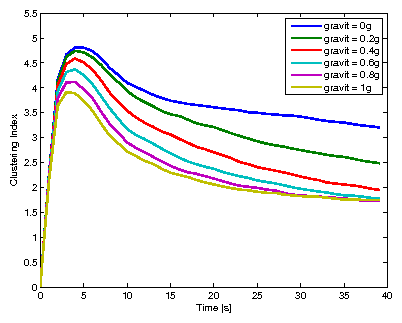
\includegraphics[width=0.45\textwidth]{Figures/gravity_time_decay}
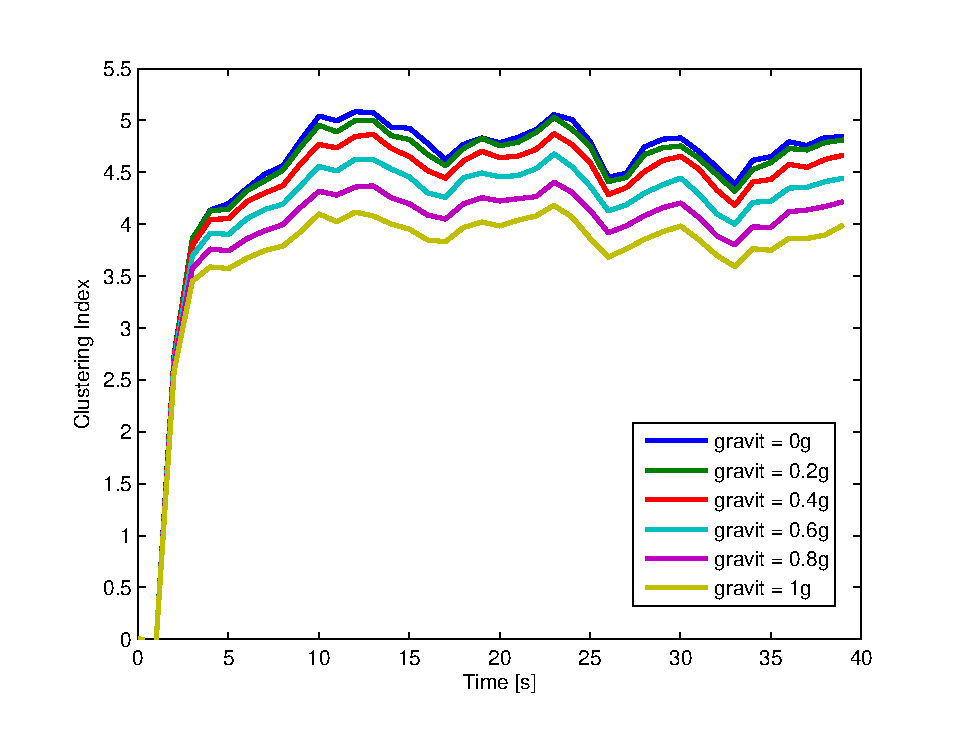
\includegraphics[width=0.45\textwidth]{Figures/gravity_time_force}
\caption{Time evolution of clustering index with different sedimentation term in decaying turbulence (see left) and
forced turbulence (see right figure).}
\label{fig:gravity_cluster}
\end{figure}

\begin{figure}\centering
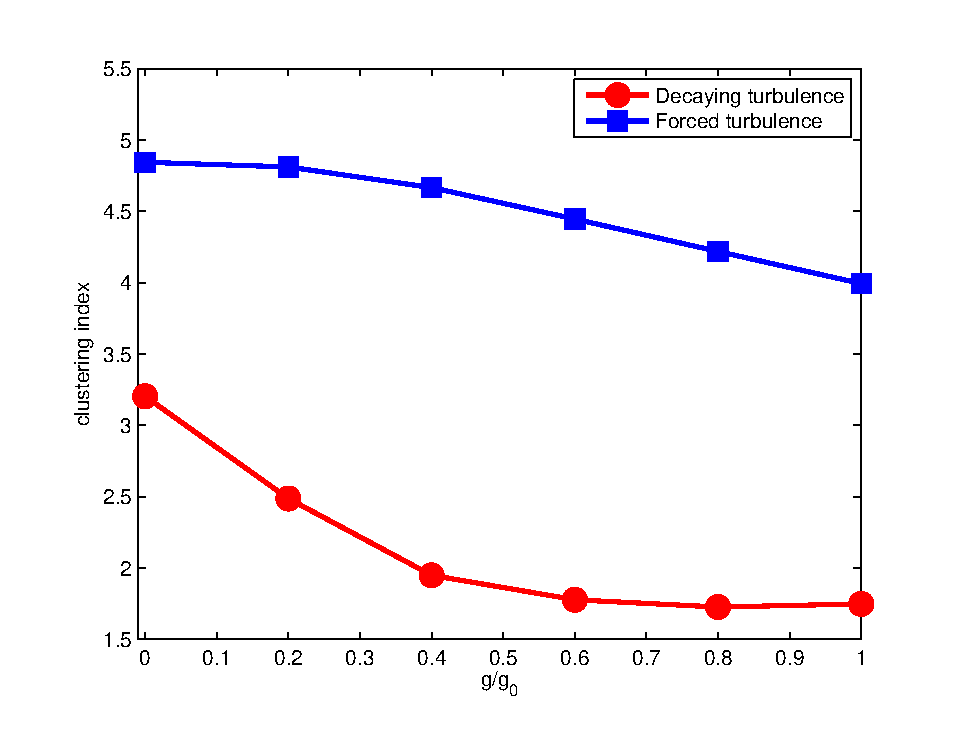
\includegraphics[width=0.8\textwidth]{Figures/sedwithgravity}
\caption{Clustering index as a function of gravitational accleration. The parameters are normalized by the original gravitational accerlation $g_0 = 9.8m/s^2$.}\label{fig:sed_gravity}
\end{figure}

\begin{figure}\centering
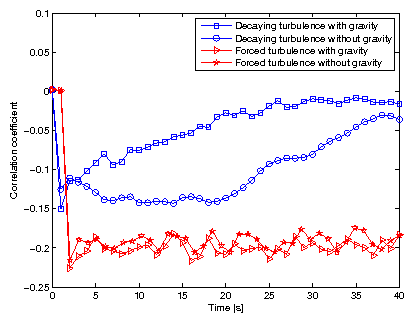
\includegraphics[width=0.8\textwidth]{Figures/correlation} \caption{Correlation
coefficient between vorticity magnitude and droplet number density as a
function of time. The correlation coefficients are computed following the
Pearson product-moment correlation coefficients, which measures the linear
correlation between two variables with positive and negative correlations
inclusive.\label{fig:correlation}} \end{figure}

\section{Summary}
In this paper, a series of numerical simulation is performed to study the cloud
entrainment and mixing phenomena. Three different configurations are compared
with each other to inspect the influence of the initial cloudy shape on the
cloud microphysics in the mixing process. The simulation duplicates the
configurations in \cite{And04} and \cite{Kumar11} and agrees with their main
results. Case 1 corresponds to \cite{And04}, which is aiming to study the final
stage of the mixing process. Case 2 tries to mimic the idealized cloud slab in
\cite{Kumar11}, presenting a complete view of entrainment and mixing. Case 3 is
created by rotating case 2 with $90$ degree clockwise to show the sedimentation
effects on the droplet spectrum.

The work described in this paper almost follows the configurations in
\cite{Kumar11}. However, due to the Gibb's phenomena of the pseudo-spectral
method, there is an inconsistency between the initial profile of cloud droplets
and vapor mixing ratio in \cite{Kumar11}, in which an artificial continuous
function was used to connect the area of cloudy air and clear air, while the
cloud droplets were treated as a simple slab. This inconsistency is not
desirable and can be overcome by taking advantage of the high resolution finite
difference WENO scheme, which is designed for problems with piecewise smooth
solutions containing discontinuities. Therefore, we are able to perform the
simulation with the same sharp initial interface for both cloud droplets and
the vapor mixing ratio.

All the simulation have been tested in both decaying turbulence and forced
turbulence. The thermodynamics, cloud microphysics and mixing diagram are
studied to make a comparison between different cases. The transient growth of
turbulence kinetic energy due to buoyancy effects in the decaying cases agrees
with the observation in \cite{Kumar14}. The spectrum of droplets size and
supersaturation implies that the cloudy shape effectively influence the mixing
process in decaying turbulence by affecting the reaction time and the size
distribution. However, this effect seems to be much smaller in the forced
turbulence.

The mixing diagram is then plotted to compare the $R$-$N$ relationship in
different cases, which have the same final state with zero liquid water
content. The number density in case 1 does not change for a long time due to
its already diluted configuration. This implies that the initial reductions of
number density in case 2 and 3 are due to dilution process. Case 2 is performed
to duplicate the results in \cite{Kumar14} for radius $15\mu m$ (note that
their results were amended in \cite{Kumar16Corr}). Our results disagree the
conclusion in \cite{Kumar14} but support their amendment in \cite{Kumar16Corr},
that is the mixing trajectories are not scattered around the homogeneous mixing
curve. The configuration of case 3 is the same as case 2 except the direction
of the cloud slab. The results infer that the sedimentation will accelerate the
mixing to a certain degree when comparing with case 2. Two groups of mixing
trajectories are observed in the results of case 3. We interpret the separation
of the curves as an indication that the sedimentation will push the particles
moving downwards, so as to accelerate the mixing process. The experiment
designed to test the relationship between gravity and clustering index gives a
better understanding of the sedimentation effect.
